\documentclass[10pt]{article}
\usepackage[utf8]{inputenc}
\usepackage{nicefrac}       % compact symbols for 1/2, etc.
\usepackage{microtype}      % microtypography
\usepackage{ragged2e}
\justifying
\usepackage{float}
\renewcommand{\figurename}{Rysunek}
\usepackage{natbib}
\usepackage{graphicx}
\usepackage{amsmath}
\usepackage{adjustbox}
\usepackage{polski}
\usepackage{gensymb}
\usepackage[T1]{fontenc}
\usepackage{uarialmoj}
\setcitestyle{square}

\usepackage{pdfpages}
\providecommand{\keywordspl}[1]
{
  \small	
  \textbf{\textit{Słowa kluczowe:}} #1
} 
\providecommand{\keywordseng}[1]
{
  \small	
  \textbf{\textit{Keywords:}} #1 
}
\providecommand{\dnauki}[1]
{
  \small	
  \textbf{\textit{Dziedzina nauki i techniki, zgodnie z wymogami OECD:}} #1
}


\begin{document}

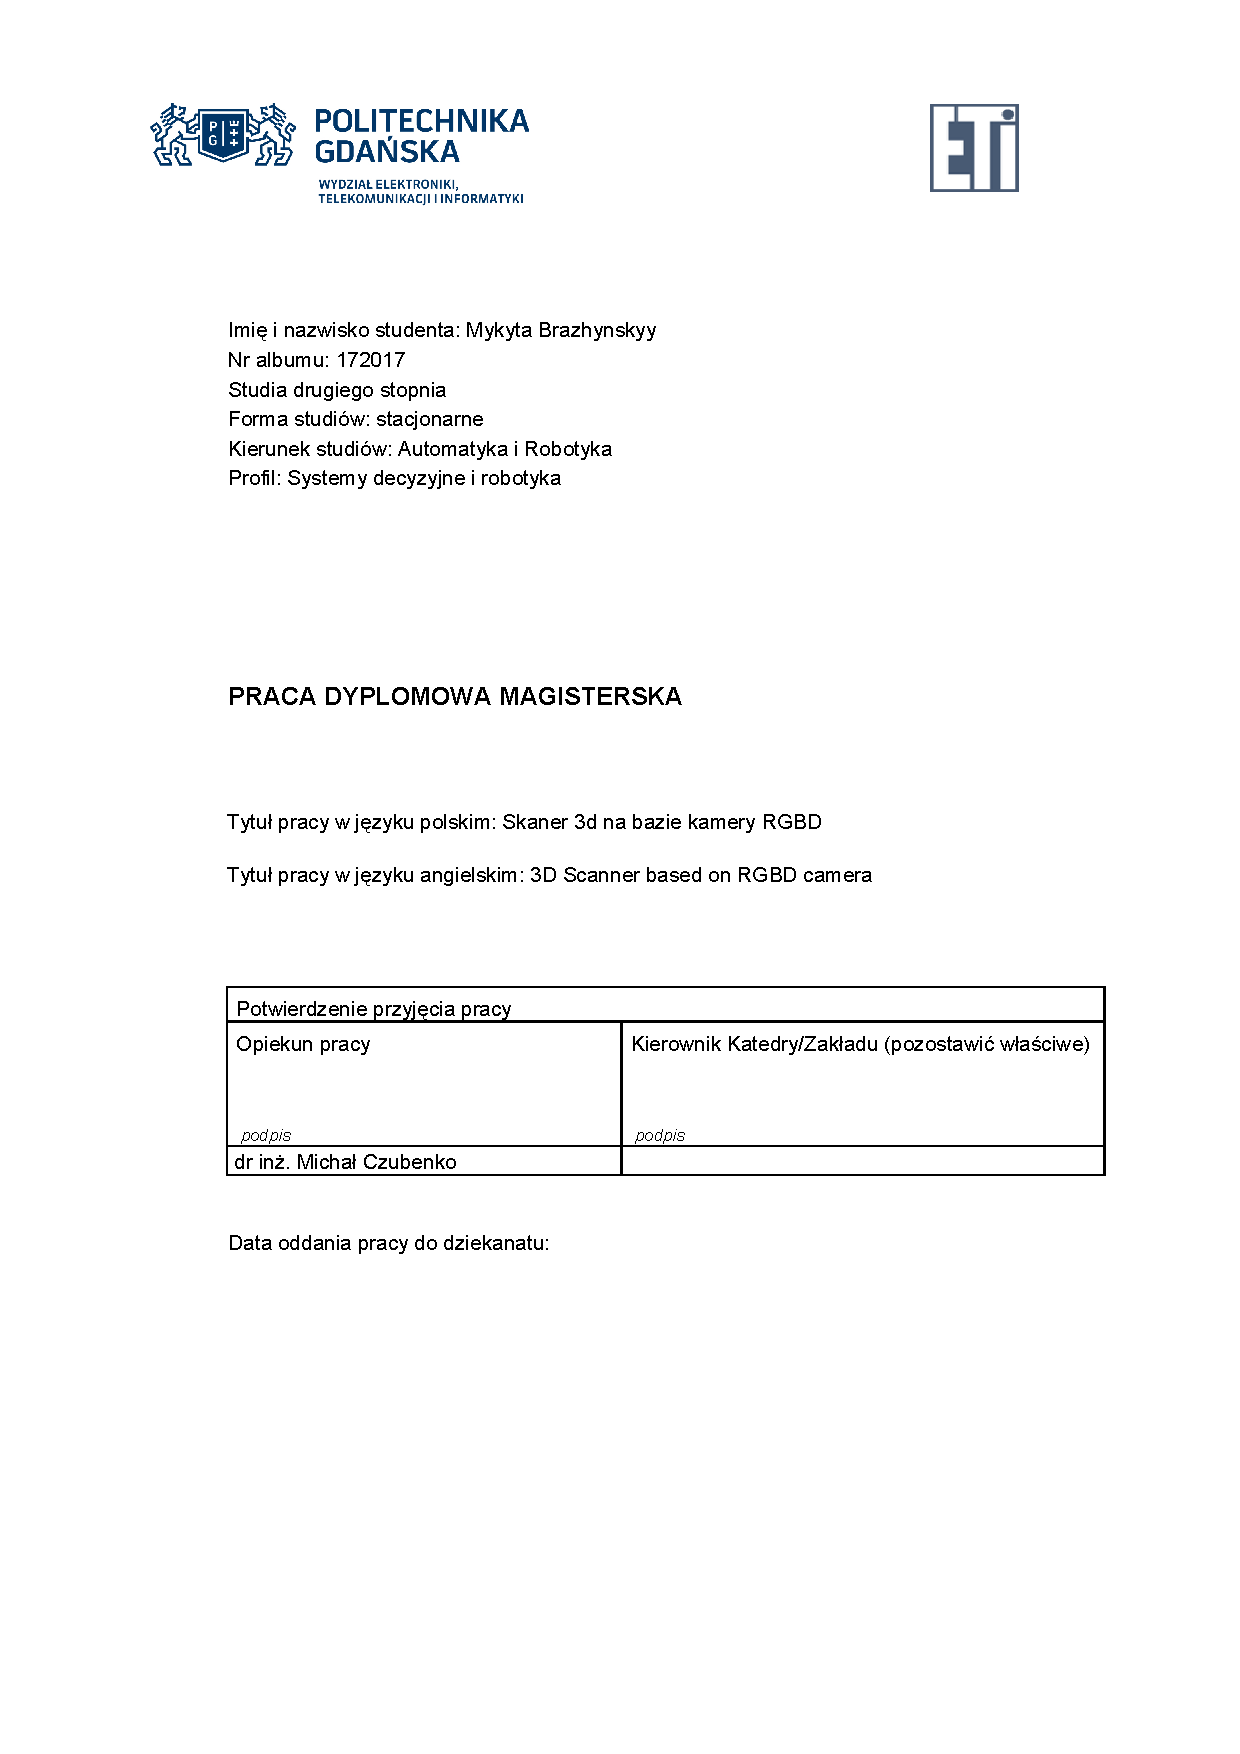
\includepdf[pages=-]{tytolowanowa.pdf}
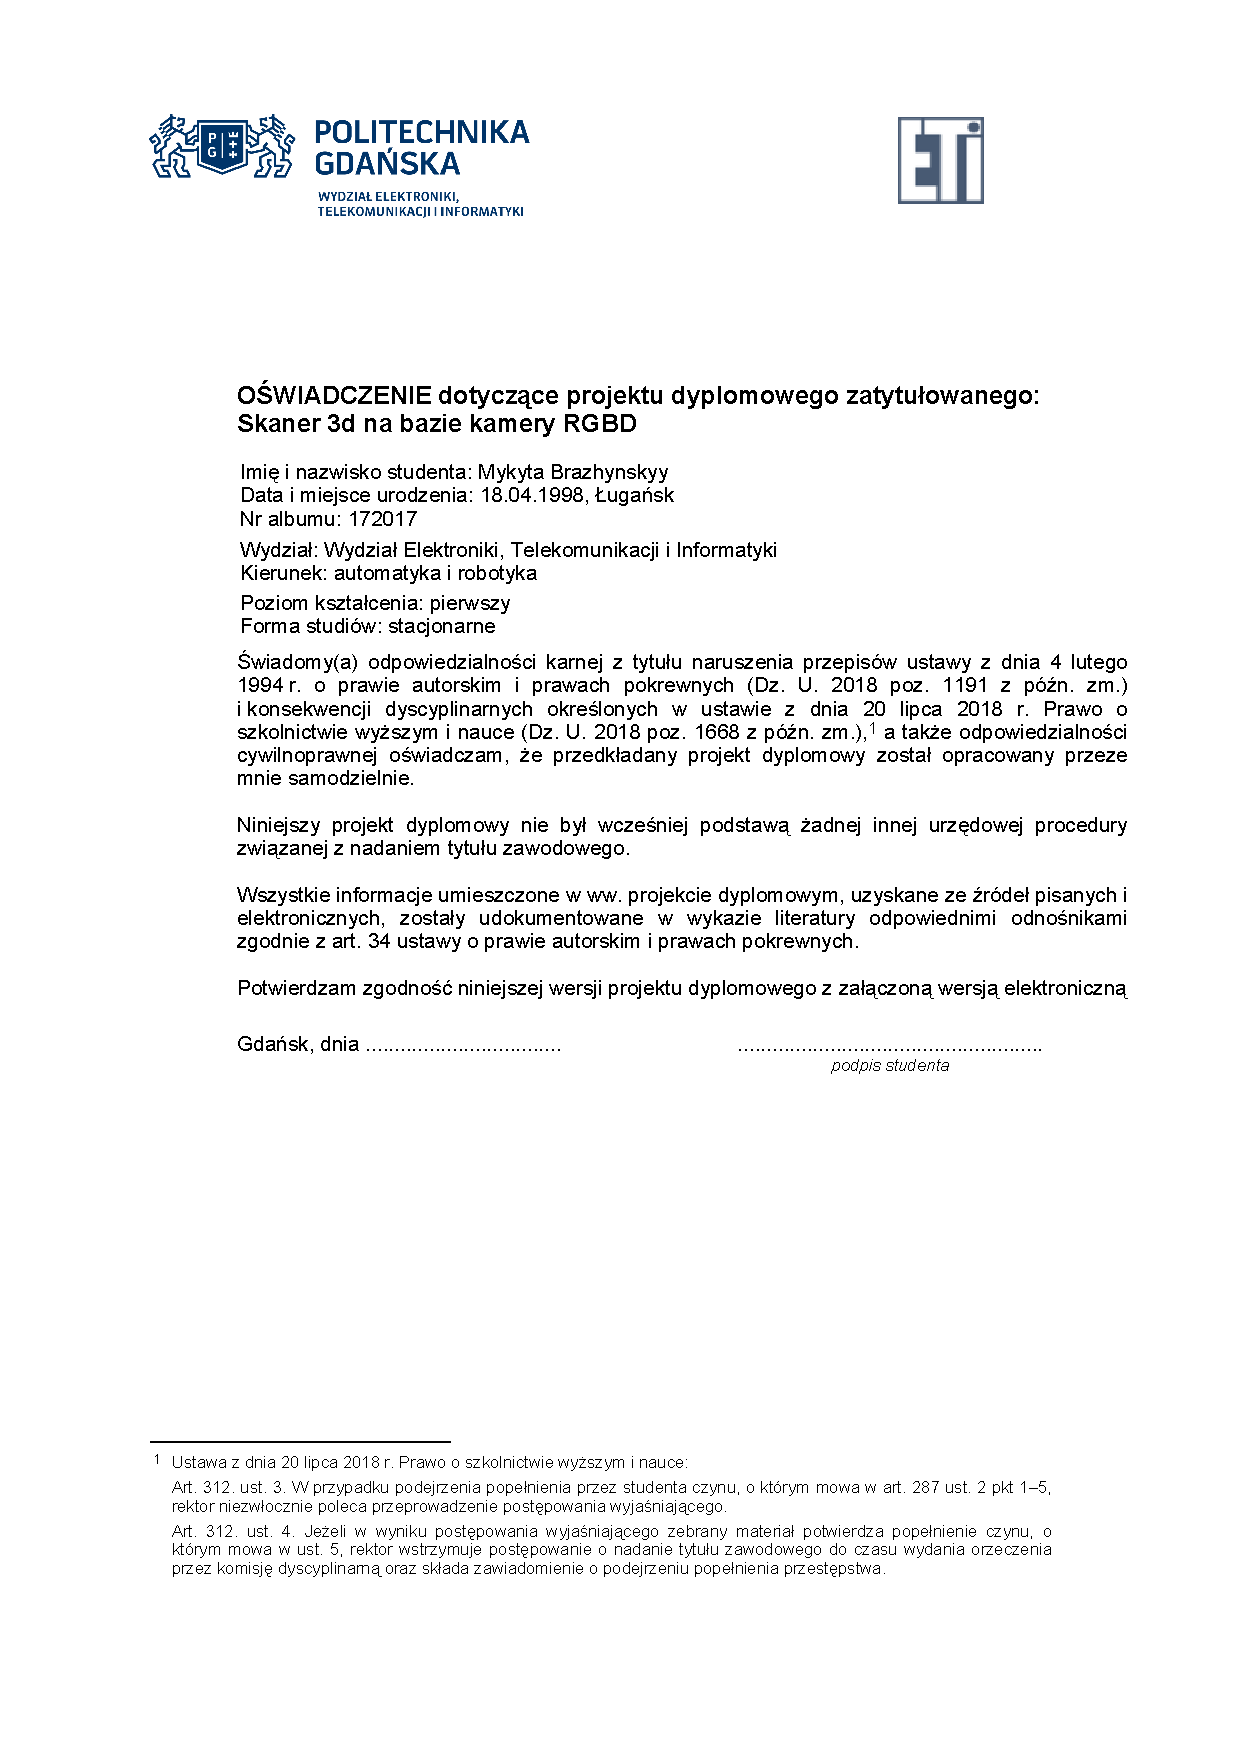
\includepdf[pages=-]{oswiadczenie.pdf}


\newpage

 
\section*{STRESZCZENIE}
Celem niniejszej pracy dyplomowej było stworzenie skanera 3D oraz systemu wizualizacji utworzonych modeli rzeczywistych obiektów. Do budowy urządzenia wykorzystano kamerę głębi firmy Intel o nazwie RealSense D435i. W pracy został przedstawiony sposób budowy skanera 3D, jego kalibracji oraz algorytmy służące do przetwarzania otrzymanych danych pomiarowych w celu uzyskania wirtualnych modeli. W celu łatwiejszej obsługi programu został utworzony interfejs graficzny zawierający najważniejsze parametry wizualizacji i obróbki danych. Na koniec dane są eksportowane do modeli w formacie obsługiwanym przez program Blender.

\keywordspl{Skaner 3D ,Intel RealSense, Python, Kamera RGBD}

\dnauki{Nauki inżynieryjne i techniczne, Systemy automatyzacji i kontroli }

\section*{ABSTRACT}
The aim of this thesis was to create a 3D scanner and a system for visualization of created models based on real objects. In the work is presented how to build a 3D scanner, its calibration and algorithms used to process the obtained measurement data to obtain virtual models. In order to make the program easier to use, a graphic interface was created containing the most important parameters of visualization and data processing. Finally, the data are exported to the models in a format supported by the Blender program.

\keywordseng{3D Scanner, Intel RealSense, Python, RGBD Camera}
\newpage
\tableofcontents





\newpage
\section{WYKAZ WAŻNIEJSZYCH OZNACZEŃ I SKRÓTÓW}

Kamera RGBD-Kamera głębi, oprócz wykonywania zdjęć RGB potrafi ona również dokonać pomiaru odległości od obiektów i nanieść te informację na powierzchnię poszczególnych pikseli obrazu.\\
LIDAR-ang.(Light Detection And Ranging) urządzenie służące do dokładnego pomiaru odległości. Działaniem przypomina funkcjonowanie radaru, lecz korzysta z odliczania czasu przelotu światła lasera, a nie mikrofal.

\section{WSTĘP I CEL PRACY}
\subsection{Wprowadzenie}
Rozwój druku 3D zwiększył zapotrzebowanie na szczegółowe metody modelowania obiektów 3D. Jedną z takich metod jest trójwymiarowy skan rzeczywistego obiektu, a następnie przeniesienie go do wirtualnego systemu komputerowego. Istnieje wiele rozwiązań na rynku pozwalających na utworzenie precyzyjnych trójwymiarowych modeli. Duża część z nich pozwala na eksport takich modeli do formatów obsługiwanych przez program Blender. Niestety większość z nich jest płatna oraz ma mało możliwości konfiguracji poszczególnych parametrów związanych z rekonstrukcją kształtu obiektów. W niniejszej pracy zostanie zaprezentowany sposób na wierne utworzenie obiektu 3D ze skanów zrobionych za pomocą kamery Intel RealSense D435i. Wybór tematu pracy nie jest losowy, ponieważ ta technologia inspiruje mnie od dłuższego czasu i zależy mi, aby te metody były przede wszystkim ogólnodostępne oraz bezpłatne.
\subsection{Cele i założenia}
Celem niniejszej pracy jest zaprojektowanie skanera 3D oraz wyeksportowanie kolorowych modeli do programu Blender przy zastosowaniu kamery Intel RealSense D435i.
Ukazane zostaną również metody analizy oraz obróbki danych, które mają posłużyć do cyfrowej implementacji rzeczywistych obiektów zmierzonych przez kamerę RGBD. Część teoretyczna polega na zobrazowaniu istniejących rozwiązań zagadnienia. Wyjaśniono algorytmy służące do przetworzenia danych uzyskanych z kamery głębi w chmurę punktów. Wymieniony został określony ciąg czynności pozwalających na dodanie na chmurę punktów siatki oraz tekstur. W części praktycznej zostaną ukazane metody kalibracji urządzenia Intel RealSense oraz proces tworzenia wirtualnych obiektów ze skanu.
\subsection{Zawartość pracy}
Pierwszy rozdział opisuje cele oraz założenia pracy. Wykonano przegląd istniejących metod mających na celu generację trójwymiarowych obiektów na podstawie danych z kamery głębi wraz z zastosowaniami współczesnych skanerów 3D.

W kolejnym rozdziale przedstawiony jest model oraz konstrukcja skanera 3D. Przeprowadzono gruntowną analizę wpływu kalibracji oraz nastaw parametrów urządzenia na otrzymany efekt końcowy. Następnie przedstawiono opisy zastosowanych algorytmów oraz kolejność ich wykonywania na podstawie autorskiego programu w języku Python. W końcowym etapie poddano analizie pod względem dokładności rezultaty pomiarów w porównaniu do rzeczywistych wartości mierzonych.

Trzeci rozdział zajmuje się podsumowaniem zarówno wykonanej pracy, jak i otrzymanych efektów. Ponadto porusza kwestię potencjalnych możliwości udoskonalenia urządzenia.

\subsection{Wprowadzenie do technologii skanerów 3D}

Początki skanerów 3D datuje się na lata 60 XX wieku. Do uzyskania modeli używano wówczas światła, kamer oraz projektorów. Niestety, wymagania dotyczące nakładu pracy nie były proporcjonalne do otrzymanych wyników, których dokładność była względnie niska. W połowie lat 80-tych komputery zyskały na popularności, a narzędzia pomiarowe stały się dokładniejsze w efekcie czego postanowiono użyć sondy stykowej. Mierzono odkształcenie sondy po zetknięciu się z obiektem wskutek czego można było wyznaczyć położenie punktów na płaszczyźnie obiektu w innym układzie współrzędnych \cite{abdel20113d}. Jej użycie pozwoliło na znaczne zwiększenie dokładności pomiarów, jednak prędkość ich wykonywania była powolna. Wobec tego zaistniała zauważalna potrzeba opracowania metody optycznej, która umożliwiłaby mierzenie obiektów z większą prędkością. Miałoby to na celu również pomiar elastycznych przedmiotów, które dotychczas nie były mierzalne ze względu na użyte technologie. Istnieje wiele różnych podejść do trójwymiarowych skanerów, każde z nich ma zastosowanie w określonej dziedzinie. Poniżej przedstawiono najważniejsze z nich.

\paragraph{Metoda triangulacji laserowej\newline}
Występują dwa typy skanerów korzystających z danej metody pomiarowej. W pierwszym typie takiego skanera układ pomiarowy składa się z nadajnika laserowego, obiektu pomiarowego oraz kamery. Poprzez przesuwanie wiązki po nieruchomym obiekcie, znając położenie kamery oraz korzystając ze wzorów \cite{mikulski2013metody} można wyznaczyć położenie zmierzonych punktów w docelowym układzie współrzędnych. Zaletami tej konstrukcji są dokładność i wysoka rozdzielczość \cite{nowacki2018pomiar}. Skanery te jednak nie sprawdzają się przy rekonstrukcji błyszczących oraz przezroczystych powierzchni. Zasada działania skanera została przedstawiona na rysunku poniżej.

\begin{figure}[H]
  \centering
  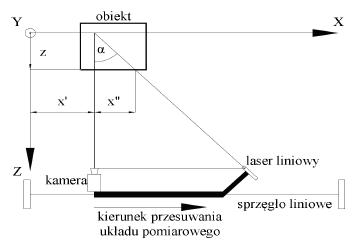
\includegraphics[scale=0.75]{skaner_triangulacja.png}
  \caption{Schemat skanera wykorzystującego triangulację laserową \cite{mikulski2013metody}}   
  \label{fig:picture}
\end{figure}

Posługując się poniższymi wzorami można uzyskać współrzędne przestrzenne mierzonego obiektu, co w rezultacie pozwala na jego odwzorowanie w komputerowej symulacji.


    


\begin{equation}
    \begin{aligned}
        & x''=k_{x} *x_{pic}\\
        & \ X=x+x'' \\
      & Y=k_{y}+y_{pic} \\
      & Z=ctg\alpha *x''\\
          
    \end{aligned}
\end{equation}

Gdzie:\\
\hspace*{3em}
\begin{tabular}{rl}
    X,Y,Z:& są współrzędnymi przestrzennymi zmierzonego obiektu. \\
    X':& położenie kamery względem początku ramienia uchwytu. \\
    X'':& wynik pomiaru w kierunku osi X w docelowych jednostkach. \\
    \alpha:& kąt pomiędzy płaszczyzną linii lasera,a płaszczyzną obrazu. \\
    $x_{pic},y_{pic}$:& współrzędne linii lasera w pikselach. \\
    $k_{x},k_{y}$:& skala przejścia z pikseli na docelowe jednostki miary. \\
\end{tabular}
\newline
\newline
Drugi typ skanerów opartych o metodę triangulacji laserowej steruje położeniem obiektu względem lasera.Korzystając z tego rozwiązania, możliwe jest uzyskanie dokładniejszych wyników oraz odwzorowanie bardziej skomplikowanych kształtów. W skład elementów konstrukcyjnych takiego układu wchodzą laser, kamera oraz tacka obrotowa z umieszczonym na niej obiektem pomiarowym.
W przeciwieństwie do skanera pierwszego typu, w tym układzie kamera oraz laser są nieruchome. Porusza się jedynie tacka obrotowa z obiektem. Laser wyświetla pionową linię na obiekt, a kamera rejestruje ten obraz. Tacka obracana jest o stały kąt d$\theta$. Po zmierzeniu kąta nachylenia α pomiędzy kamerą, a laserem jak również kąta nachylenia β kamery względem tacki można dokonać transformacji ze współrzędnych obiektu do współrzędnych obrazu przechodzących przez oś obrotu podstawy. Schemat działania takiego urządzenia został przedstawiony poniżej.

\begin{figure}[H]
  \centering
  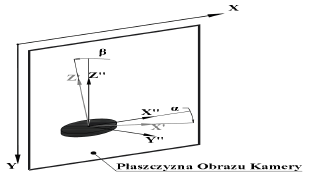
\includegraphics[scale=0.75]{skanerPionowaLinia.png}
  \caption{Układ współrzędnych nieruchomego skanera \cite{mikulski2013metody}}   
  \label{fig:picture}
\end{figure}
\newline
Współrzędne zmierzonego obiektu w układzie kamery można opisać poniższymi równaniami.

\begin{equation}
    \begin{aligned}
        & \ Z''=y_{0}-(y-(x'-x_{0}))tan\alpha \\
          & X''=x-x_{0}+(y'-y_{0})tan\beta \\
          & Y''=0\\
    \end{aligned}
\end{equation}
Gdzie:\\
\hspace*{3em}
\begin{tabular}{rl}
    X,Y:& są współrzędnymi obrazu kamery w pikselach. \\
    X',Z':& układ współrzędnych linii emitowanej przez laser. \\
    $\alpha$:& kąt nachylenia linii lasera do płaszczyzny obrazu. \\
    $\beta$:& kąt nachylenia docelowego układu współrzędnych do płaszczyzny obrazu. \\
    $x_{0},y_{0}$:& współrzędne środka tacki w pikselach. \\
    X'',Y'',Z'':& docelowy układ współrzędnych. \\
\end{tabular}
\newline
Ostatecznie korzystając z macierzy obrotu względem osi Z'' można uzyskać współrzędne chmury punktów.


\centerline{
\begin{bmatrix}
    X''' \\
    Y''' \\
    Z''' \\
\end{bmatrix}
=
\begin{bmatrix}
    cos\theta & -sin\theta & 0\\
     sin\theta & cos\theta & 0\\
    0 & 0 & 1
\end{bmatrix}
\begin{bmatrix}
    X''\\
     Y''\\
    Z''
\end{bmatrix}

}
    


Gdzie:\\
\hspace*{3em}
\begin{tabular}{rl}
    $\theta$:& kąt obrotu tacki. \\
    X'',Y'',Z'':& układ współrzędnych kamery. \\
    X''',Y''',Z''':& układ współrzędnych chmury punktów. \\
\end{tabular}

Na rynku istnieje wiele skanerów trójwymiarowych wykorzystujących metodę triangulacji laserowej. Poniżej zostaną omówione charakterystyki jednego z nich.

\begin{figure}[H]
  \centering
  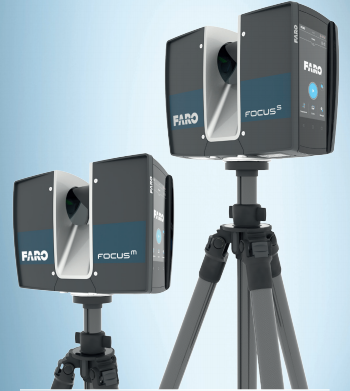
\includegraphics[scale=0.70]{farofocus.PNG}
  \caption{Skaner Faro Focus S350}   
  \label{fig:picture}
\end{figure}

\begin{table}[H]
\begin{center}

\caption{\label{tab:tab2}Charakterystyki skanera Faro Focus S350 \cite{farofocusDatasheet}.}
\centerline{
\begin{tabular}{ |c| c| }
 \hline
 {\bf Zasięg} & 0.6m-350m\\ 
  \hline
 {\bf Błąd pomiaru odległości} & $\pm$1mm\\  
 \hline
 {\bf Prędkość pomiaru} & do 976000 $\frac{pkt}{s}$ \\  
  \hline
 {\bf Dokładność kątowa} & Do 19 sekund kątowych  \\  
  \hline
   {\bf Dokładność pozycji 3D} & 3.5 mm  \\  
  \hline
     {\bf Długość fali lasera } & 1550nm  \\  
  \hline

\end{tabular}
}

\end{center}
\end{table}

\paragraph{Metoda emitowania światła strukturalnego\newline}

Skanery oparte na tej metodzie wyświetlają siatkę świetlną na mierzony obiekt. Następnie wzór na obiekcie jest mierzony przez jedną lub dwie kamery. Za sprawą badania mocy światła odbitego oraz kształtu siatki na przedmiocie, korzystając z metod triangulacji, można wyznaczyć położenie obiektu w innym układzie współrzędnych. Jednocześnie wskutek wykorzystania obrazu z dwóch kamer jest możliwe wykonanie pełnego zdjęcia 3D. Głównym walorem tej metody jest szybka prędkość działania, ponieważ zdjęcia mogą być wykonywane z dużą częstotliwością. Ponadto światło emitowane przez ten skaner nie jest światłem laserowym, dlatego też wszelkie aspekty zagrażające wzrokowi są wyeliminowane. Słabym punktem tej metody jest ograniczona gęstość rzutowanej siatki. Co w przypadku obiektu o skomplikowanym kształcie sprawia,iż pomiar będzie musiał być wykonany parokrotnie pod różnymi kątami w celu uzyskania dokładnych wyników \cite{nowacki2018pomiar}. Zasada działania skanera bazującego na metodzie emitowania światła strukturalnego została przedstawiona na rysunku poniżej.

\begin{figure}[H]
  \centering
  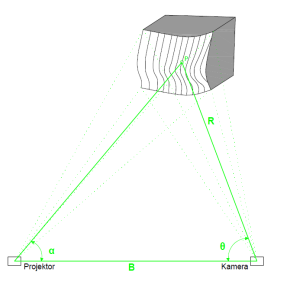
\includegraphics[scale=0.75]{swiatlostrukturalne.PNG}
  \caption{Metoda wyznaczania współrzędnych w technice światła strukturalnego \cite{Wrona_Piotrowska_2015}}   
  \label{fig:picture}
\end{figure}
\newline
Korzystając z podstawowych zależności trygonometrycznych możliwe jest wyprowadzenie równań pozwalających na wyznaczenie odległości poszczególnych punktów mierzonego obiektu od kamery.
\begin{equation}
    \begin{aligned}
        & \frac{R}{sin\alpha}=\frac{B}{sin(180-\alpha-\theta)} \\
          & R=B\frac{sin\theta}{sin(\alpha+\theta)} \\
    \end{aligned}
\end{equation}

Gdzie:\\
\newline
    $\alpha$:& kąt pomiędzy wiązką światła emitowanego prze projektor, a odcinkiem łączącym projektor oraz kamerę. \\
    $\theta$:& kąt pomiędzy wiązką światła docierającą do kamery, a odcinkiem łączącym projektor oraz kamerę. \\
    B:& odległość pomiędzy kamerą, a projektorem. \\
    R:& odległość kamery od mierzonego przedmiotu. \\

Poniżej został przedstawiony skaner wykorzystujący technologię emitowania światła strukturalnego.

\begin{figure}[H]
  \centering
  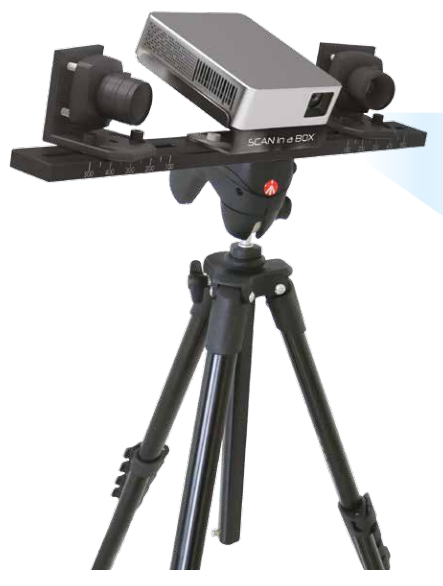
\includegraphics[scale=0.50]{siobimg.PNG}
  \caption{Skaner Faro Scan in a box}   
  \label{fig:picture}
\end{figure}

W skład skanera wchodzą dwie kamery odbierające informację o tym, jaki jest rozkład siatki świetlnej na obiekcie oraz emiter rzutujący odpowiedni wzór na przedmiot.

\begin{table}[H]
\begin{center}

\caption{\label{tab:tab2}Charakterystyki skanera Faro Scan in a box \cite{siabDatasheet}.}
\centerline{
\begin{tabular}{ |c| c| }
 \hline
 {\bf Zasięg} & 0.2m-1.12m\\ 
  \hline
 {\bf Gęstość siatki} & 0.078mm-0.39mm\\  
 \hline
 {\bf Prędkość pomiaru} & $<4$s \\  
  \hline
 {\bf Gęstość meshu} & Do 10 mln wierzchołków  \\  
  \hline
   {\bf Dokładność } & Do  0.1 \% wielkości obiektu \\  
  \hline

\end{tabular}
}

\end{center}
\end{table}


\paragraph{Fotogrametria\newline}

Jest to metoda odtwarzania trójwymiarowego kształtu obiektów z płaskich dwuwymiarowych zdjęć. Polega ona na mierzeniu korelacji między sobą poszczególnych obrazów, które wykonywane są w odstępie od 5 do 15 stopni od siebie. W celu zwiększenia dokładności używa się również technologii SFM ( ang. Structure From Motion). Opiera się ona na identyfikacji homologicznych punktów na różnych obrazach w celu uzyskania perspektywy między nimi. Poprzez wykorzystanie efektu paralaksy istnieje możliwość późniejszego określenia w jakiej odległości od kamery znajdywały się poszczególne punkty na obrazie. Umożliwia to utworzenie funkcji przejścia między nimi oraz otrzymanie na końcowym etapie pełnego modelu 3D \cite{glowienka2015fotogrametria}. Pozytywnym aspektem tego rozwiązania jest niski koszt, gdyż do wykonania zdjęć wystarczy jedynie aparat w urządzeniu mobilnym. Największą wadą jest wysoka złożoność obliczeniowa. Często takie obliczenia wykonywane są w chmurze co zwiększa koszty eksploatacji takiej metody oraz dokładność pomiarów jest względnie niska w porównaniu ze skanerami RGBD.

\paragraph{Skanery impulsowe LIDAR\newline}

Zasada działania takiego lasera jest zbliżona do funkcjonowania radaru. Skanery impulsowe mierzą czas potrzebny wiązce lasera do przebycia drogi do przedmiotu i na tej podstawie określają odległość zmierzonego punktu od  źródła światła. Skanery te wykorzystuje się do mierzenia dużych odległości, ponieważ zmierzenie czasu lotu światła na małych odległościach jest wysoce trudne do zrealizowania. Dużym ograniczeniem tego typu rozwiązania jest pomiar tylko jednego punktu na obiekcie przy jednym cyklu, dlatego też wykonanie pełnego skanu obiektu trwa znacznie dłużej niż w innych skanerach. Jednakże jedynie ta metoda zapewnia wymierne rezultaty na duże odległości.
\newline
Istnieją dwa typy skanerów LIDAR \cite{wehr1999airborne}:\\
\textbf{1.}Mierzący czas od momentu wysłania wiązki światła, aż do jej odbicia od obiektu ang.(TOF-time of flight). Zasada działania takiego skanera polega na wysłaniu wiązki światła w kierunku obiektu, a następnie zmierzenie w jakim czasie wiązka wróci do odbiornika. Takie urządzenia, ze względu na swoją konstrukcję i bardzo dobrą dokładność na dużych odległościach są stosowane najczęściej \cite{introToLidar}.

Przykładem takiego instrumentu pomiarowego jest Benewake TF03 przestawiony poniżej.

\begin{figure}[H]
  \centering
  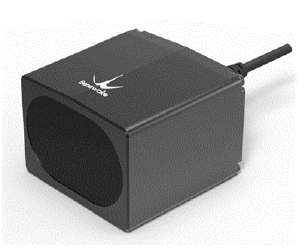
\includegraphics[scale=0.60]{benewaketf03img.PNG}
  \caption{Skaner Benewake TF03-180}   
  \label{fig:picture}
\end{figure}

\begin{table}[H]
\begin{center}

\caption{\label{tab:tab2}Charakterystyki skanera Benewake TF03-180 \cite{benewaketf03}.}
\centerline{
\begin{tabular}{ |c| c| }
 \hline
 {\bf Zasięg} & 0.1m-180m\\ 
  \hline
   {\bf Dokładność } &Do 1cm   \\  
  \hline
     {\bf Prędkość pomiaru } &Do 1000Hz   \\  
  \hline
   {\bf  Długość fali lasera } & 905nm   \\  
  \hline
     {\bf  Kąt wykrycia wiązki światła  } & 0.5\degree   \\  
  \hline
    
   {\bf Błąd pomiaru } & $\pm$10cm przy ogległości do 10m,1\% powyżej 10m  \\  
  \hline

\end{tabular}
}

\end{center}
\end{table}

\textbf{2.}Mierzący przesunięcie fazowe wiązki odbitej od obiektu ang.(Phase-based LIDAR). Główną zasadą wykorzystywaną w tym skanerze jest fakt, że przy odbiciu od powierzchni faza światła zostaje przesunięta. Mając również na uwadze, iż różnica przesunięcia fazowego pomiędzy wiązką odbitą, a wiązką wysłaną jest proporcjonalna do odległości przebytej przez światło można otrzymać następujące wzory \cite{articleLidar}.

\begin{equation}
    \begin{aligned}
       d=\frac{c}{2f}* \frac{\phi}{2\pi}\\
    \end{aligned}
\end{equation}

Gdzie:\\

\hspace*{3em}
\begin{tabular}{rl}
    d:& odległość zmierzonego punktu od odbiornika \\
    c:& prędkość światła. \\
    $f$:& częstotliwośc sygnału referencyjnego. \\
    $\phi$:& przesunięcie fazowe pomiędzy sygnałem referencyjnym, a odebranym przez odbiornik. \\
\end{tabular}\\
Z powyższego wzoru wynika również fakt, że w celu uzyskania dokładniejszych pomiarów odległości należy zwiększyć częstotliwość światła służącego do próbkowania.\newline
\newline
Skaner Benewake TF02 jest urządzeniem wykorzystującym pomiar przesunięcia fazowego do obliczania odległości ang. (indirect time-of-flight). Jego charakterystyki oraz wygląd zostały przedstawione poniżej.

\begin{figure}[H]
  \centering
  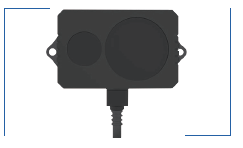
\includegraphics[scale=0.75]{benewaketf02img.PNG}
  \caption{Skaner Benewake TF02}   
  \label{fig:picture}
\end{figure}

\begin{table}[H]
\begin{center}

\caption{\label{tab:tab2}Charakterystyki skanera Benewake TF02 \cite{benewaketf02}.}
\centerline{
\begin{tabular}{ |c| c| }
 \hline
 {\bf Zasięg} & 0.4m-22m\\ 
  \hline
   {\bf Dokładność } &Do 1cm   \\  
  \hline 
     {\bf Prędkość pomiaru } &Do 100Hz   \\  
  \hline
   {\bf  Długość fali lasera } & 850nm   \\  
  \hline
     {\bf  Kąt wykrycia wiązki światła  } & 3\degree   \\  
  \hline
    
   {\bf Błąd pomiaru } & $\pm$5cm przy ogległości do 5m,2\% powyżej 5m  \\  
  \hline

\end{tabular}
}

\end{center}
\end{table}
\newline
Obie te metody, zarówno pomiaru przesunięcia fazowego jak i mierząca czas przelotu światła charakteryzują się bardzo dobrą dokładnością. Jednak znajdują zastosowanie w różnych dziedzinach. Skanery LIDAR pierwszego typu stosuje się przy pomiarach daleko zasięgowych, głównie w terenie. Natomiast te drugiego typu wykorzystywane są przy pomiarach krótko-zasięgowych wymagających wysokiej dokładności oraz szybkości działania. Dlatego stosowane są głownie w pomiarach różnego typu odkształceń \cite{usageOfLidar}.
\paragraph{Ogólne charakterystyki laserowych metod pomiarowych\newline}

Zestawienie uśrednionych parametrów poszczególnych metod pomiarowych znajduje się w tabeli poniżej.
\begin{table}[H]
\begin{center}
\caption{\label{tab:tab2}Charakterystyki metrologiczne laserowych metod pomiarowych \cite{nowacki2018pomiar}.}
\centerline{
\begin{tabular}{ |c| c|c|c| } 
 \hline
 \bf {Metoda pomiarowa} & \bf {Zakres pomiarowy [m]} & \bf{Dokładność [mm]}& \bf {Szybkość  $\frac{punkty}{sekunda}$ } \\ 
  \hline
 Metoda pomiaru czasu lotu impulsu & $<1500$ & $<20$ & Do 12000 \\  
  \hline
 Metoda przesunięcia fazowego & $<100$   & $<10$   & Do 625000  \\
   \hline
 Triangulacja & $<5$ & $<0.1$  & Do 10000 \\
 \hline
 
\end{tabular}

}

\end{center}
\end{table}



\paragraph{Zastosowania skanerów 3D\newline}

Współcześnie skanery 3D mają zastosowanie w większości gałęzi życia oraz przemysłu. Przemysł budowlany wykorzystuje je w celu mierzenia odkształceń belek z dużą dokładnością \cite{goszczynska2014doswiadczalna}. W medycynie mogą być użyte do skanowania części ciała oraz modelowania komputerowego kończyn \cite{tomaka20053d}. Wykorzystywane są również przy oględzinach pacjentów. Wysoka dokładność przy mierzeniu odkształceń na powierzchni ciała sprawia, że dzięki skanerom 3D można dostrzec złamania kości oraz inne ubytki \cite{thali2003optical}.Kolejną ważną rolą, jaką spełniają skanery 3D w służbie zdrowia jest druk 3D. Poprzez analizę danych otrzymanych z trójwymiarowych pomiarów oraz drukarki 3D można tworzyć modele kończyn. Takie elementy są pomocne przy nauce studentów oraz znajdują swoje zastosowanie w protetyce \cite{mcmenamin2014production}. Również w przemyśle spożywczym skanery 3D używane są do kontroli jakości poszczególnych wyrobów \cite{anders2012zastosowanie}.

\addcontentsline{toc}{section}{Bibliografia}
\bibliography{references}
\bibliographystyle{ieeetr}
\end{document}
